\documentclass[tikz,border=6pt]{standalone}
\usepackage{tikz}
\usetikzlibrary{arrows.meta,backgrounds,calc,fit,positioning,shapes.geometric,shapes.misc}

\definecolor{macroblue}{HTML}{4C78A8}
\definecolor{midgreen}{HTML}{59A14F}
\definecolor{microorange}{HTML}{F28E2B}
\definecolor{softgray}{HTML}{F4F4F4}
\definecolor{chipgray}{HTML}{E4E6E8}
\definecolor{edgegray}{HTML}{B8BDC3}
\definecolor{textgray}{HTML}{4D4D4D}

\colorlet{hiddenflowcolor}{macroblue!92!black}
\colorlet{featureflowcolor}{microorange!95!black}
\colorlet{metaflowcolor}{black!55}

\tikzset{
  >={Latex[length=2.5mm,width=2.2mm]},
  every node/.style={inner sep=0pt,outer sep=0pt},
  figure label/.style={font=\scriptsize\sffamily\bfseries,text=textgray},
  section label/.style={font=\scriptsize\sffamily,text=textgray},
  band text/.style={font=\scriptsize\sffamily\bfseries,text=black!85,align=center},
  tokenbox/.style={rounded corners=2pt, draw=edgegray, fill=white, line width=0.6pt},
  sourcebox/.style={rounded corners=5pt, draw=edgegray, fill=white, line width=0.6pt},
  panelbox/.style={rounded corners=7pt, draw=black!12, fill=white, line width=0.7pt},
  neutralchip/.style={rounded corners=2pt, draw=edgegray!90, fill=chipgray, line width=0.45pt},
  cuepill/.style={rounded corners=3pt, draw=edgegray!90, fill=softgray, line width=0.5pt},
  legendtext/.style={font=\scriptsize\sffamily,text=textgray},
  stagehead/.style={rounded corners=4pt, line width=0.6pt},
  attnbox/.style={rounded corners=4pt, draw=edgegray!95, fill=softgray, line width=0.6pt},
  simplebox/.style={rounded corners=4pt, draw=edgegray!95, fill=white, line width=0.6pt},
  routerbox/.style={rounded corners=3pt, draw=edgegray!95, fill=softgray, line width=0.55pt},
  expertbox/.style={rounded corners=2pt, draw=edgegray!95, fill=white, line width=0.5pt},
  hiddenflow/.style={->, draw=hiddenflowcolor, line width=1.1pt},
  featureflow/.style={->, draw=featureflowcolor, line width=1.0pt, dash pattern=on 3.2pt off 1.8pt},
  metaflow/.style={->, draw=metaflowcolor, line width=0.55pt},
}

\newcommand{\fmoeTokenNode}[3]{%
  \begin{scope}[shift={({#1},{#2})}]
    \path[tokenbox] (-0.42,-0.34) rectangle (0.42,0.34);
    #3
  \end{scope}%
}

\newcommand{\fmoeBallIcon}{%
  \draw[line width=0.45pt, draw=textgray] (0,0) circle [radius=0.16];
  \draw[line width=0.35pt, draw=textgray] (-0.11,0) -- (0.11,0);
  \draw[line width=0.35pt, draw=textgray] (0,-0.11) -- (0,0.11);
  \draw[line width=0.3pt, draw=textgray] (-0.09,-0.09) -- (0.09,0.09);
  \draw[line width=0.3pt, draw=textgray] (-0.09,0.09) -- (0.09,-0.09);
}

\newcommand{\fmoeBootsIcon}{%
  \filldraw[draw=textgray, fill=black!10, line width=0.35pt]
    (-0.16,-0.03) -- (-0.02,-0.03) -- (0.02,-0.11) -- (-0.15,-0.11) -- cycle;
  \filldraw[draw=textgray, fill=black!10, line width=0.35pt]
    (0.01,0.04) -- (0.16,0.04) -- (0.19,-0.05) -- (0.02,-0.05) -- cycle;
}

\newcommand{\fmoeJerseyIcon}{%
  \filldraw[draw=textgray, fill=black!8, line width=0.35pt]
    (-0.13,0.12) -- (-0.04,0.12) -- (0,0.05) -- (0.04,0.12) -- (0.13,0.12) --
    (0.17,0.02) -- (0.09,-0.03) -- (0.08,-0.16) -- (-0.08,-0.16) -- (-0.09,-0.03) -- (-0.17,0.02) -- cycle;
}

\newcommand{\fmoeGuardIcon}{%
  \filldraw[draw=textgray, fill=black!9, line width=0.35pt]
    (0,0.16) -- (0.12,0.1) -- (0.09,-0.1) -- (0,-0.17) -- (-0.09,-0.1) -- (-0.12,0.1) -- cycle;
}

\newcommand{\fmoeSocksIcon}{%
  \filldraw[draw=textgray, fill=black!8, line width=0.35pt]
    (-0.13,0.14) rectangle (-0.04,-0.02);
  \filldraw[draw=textgray, fill=black!8, line width=0.35pt]
    (-0.04,-0.02) -- (0.03,-0.02) -- (0.03,-0.09) -- (-0.1,-0.09) -- cycle;
  \filldraw[draw=textgray, fill=black!8, line width=0.35pt]
    (0.04,0.14) rectangle (0.13,-0.02);
  \filldraw[draw=textgray, fill=black!8, line width=0.35pt]
    (0.04,-0.02) -- (0.11,-0.02) -- (0.11,-0.09) -- (-0.02,-0.09) -- cycle;
}

\newcommand{\fmoeOrderIcon}{%
  \draw[textgray, line width=0.45pt] (-0.16,0.09) -- (0.12,0.09);
  \draw[textgray, line width=0.45pt] (-0.16,0) -- (0.12,0);
  \draw[textgray, line width=0.45pt] (-0.16,-0.09) -- (0.12,-0.09);
  \fill[textgray] (-0.2,0.09) circle[radius=0.018];
  \fill[textgray] (-0.2,0) circle[radius=0.018];
  \fill[textgray] (-0.2,-0.09) circle[radius=0.018];
}

\newcommand{\fmoeClockIcon}{%
  \draw[textgray, line width=0.45pt] (0,0) circle[radius=0.15];
  \draw[textgray, line width=0.45pt] (0,0) -- (0,0.07);
  \draw[textgray, line width=0.45pt] (0,0) -- (0.06,-0.04);
}

\newcommand{\fmoeGridIcon}{%
  \foreach \x in {-0.12,0.02} {
    \foreach \y in {-0.1,0.04} {
      \path[draw=textgray, fill=black!6, line width=0.35pt] (\x,\y) rectangle +(0.1,0.1);
    }
  }
}

\newcommand{\fmoeBarsIcon}{%
  \filldraw[draw=textgray, fill=black!12, line width=0.35pt] (-0.16,-0.13) rectangle (-0.08,0.0);
  \filldraw[draw=textgray, fill=black!12, line width=0.35pt] (-0.03,-0.13) rectangle (0.05,0.08);
  \filldraw[draw=textgray, fill=black!12, line width=0.35pt] (0.10,-0.13) rectangle (0.18,0.14);
}

\newcommand{\fmoeSourceBox}[4]{%
  \begin{scope}[shift={({#1},{#2})}]
    \path[sourcebox] (-0.95,-0.36) rectangle (0.95,0.36);
    \begin{scope}[shift={(-0.52,0)}]
      #4
    \end{scope}
    \node[anchor=west, font=\scriptsize\sffamily\bfseries, text=textgray] at (-0.18,0) {#3};
  \end{scope}%
}

\newcommand{\fmoeChipGrid}[2]{%
  \begin{scope}[shift={({#1},{#2})}]
    \foreach \x/\y in {-0.26/0.12,0.26/0.12,-0.26/-0.14,0.26/-0.14} {
      \path[neutralchip] (\x-0.18,\y-0.06) rectangle +(0.36,0.12);
    }
  \end{scope}%
}

\newcommand{\fmoeStageCard}[5]{%
  \begin{scope}[shift={({#1},{#2})}]
    \path[simplebox] (-1.05,-0.72) rectangle (1.05,0.72);
    \path[draw=#3!80!black, fill=#3!16, rounded corners=4pt, line width=0.6pt] (-0.92,0.2) rectangle (0.92,0.58);
    \node[font=\scriptsize\sffamily\bfseries, text=black!88] at (0,0.39) {#4};
    \fmoeChipGrid{0}{-0.13}
    #5
  \end{scope}%
}

\newcommand{\fmoeLegendSample}[4]{%
  \draw[#2] (#1, #3) -- ++(0.9,0);
  \node[anchor=west, legendtext] at ($(#1,#3)+(1.05,0)$) {#4};
}

\newcommand{\fmoeCaption}[2]{%
  \par\noindent\parbox{#1}{\footnotesize\sffamily #2}%
}


\begin{document}
\sffamily
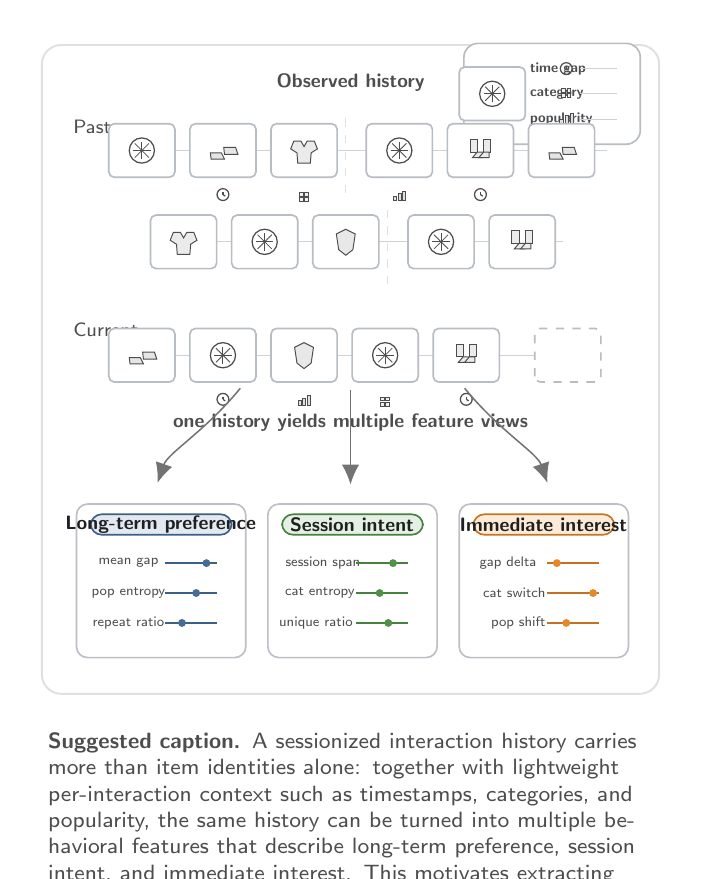
\begin{tikzpicture}[x=1cm,y=1cm]
  \path[use as bounding box] (0,-1.28) rectangle (8.3,9.18);
  \path[panelbox] (0.18,0.72) rectangle (8.02,8.96);

  \node[font=\scriptsize\sffamily\bfseries, text=textgray] at (4.1,8.48) {Observed history};

  % Small visual hint that each interaction carries both item identity and lightweight context.
  \begin{scope}[shift={(5.54,7.7)}]
    \path[sourcebox] (0,0) rectangle (2.24,1.28);
    \fmoeTokenNode{0.36}{0.64}{\fmoeBallIcon}
    \node[anchor=west, font=\tiny\sffamily\bfseries, text=textgray] at (0.84,0.96) {time gap};
    \node[anchor=west, font=\tiny\sffamily\bfseries, text=textgray] at (0.84,0.64) {category};
    \node[anchor=west, font=\tiny\sffamily\bfseries, text=textgray] at (0.84,0.32) {popularity};
    \draw[black!18, line width=0.35pt] (1.48,0.96) -- (1.94,0.96);
    \draw[black!18, line width=0.35pt] (1.48,0.64) -- (1.94,0.64);
    \draw[black!18, line width=0.35pt] (1.48,0.32) -- (1.94,0.32);
    \begin{scope}[shift={(1.3,0.96)}, scale=0.5]
      \fmoeClockIcon
    \end{scope}
    \begin{scope}[shift={(1.3,0.64)}, scale=0.46]
      \fmoeGridIcon
    \end{scope}
    \begin{scope}[shift={(1.3,0.32)}, scale=0.5]
      \fmoeBarsIcon
    \end{scope}
  \end{scope}

  % Sequence area
  \node[section label, anchor=west] at (0.58,7.92) {Past};
  \draw[black!18, line width=0.45pt] (1.1,7.62) -- (7.36,7.62);
  \fmoeTokenNode{1.45}{7.62}{\fmoeBallIcon}
  \fmoeTokenNode{2.48}{7.62}{\fmoeBootsIcon}
  \fmoeTokenNode{3.51}{7.62}{\fmoeJerseyIcon}
  \draw[black!12, dashed, line width=0.4pt] (4.04,7.08) -- (4.04,8.1);
  \fmoeTokenNode{4.72}{7.62}{\fmoeBallIcon}
  \fmoeTokenNode{5.75}{7.62}{\fmoeSocksIcon}
  \fmoeTokenNode{6.78}{7.62}{\fmoeBootsIcon}
  \begin{scope}[shift={(2.48,7.06)}, scale=0.5]
    \fmoeClockIcon
  \end{scope}
  \begin{scope}[shift={(3.51,7.02)}, scale=0.48]
    \fmoeGridIcon
  \end{scope}
  \begin{scope}[shift={(4.72,7.04)}, scale=0.46]
    \fmoeBarsIcon
  \end{scope}
  \begin{scope}[shift={(5.75,7.06)}, scale=0.5]
    \fmoeClockIcon
  \end{scope}

  \draw[black!18, line width=0.45pt] (1.62,6.46) -- (6.8,6.46);
  \fmoeTokenNode{1.98}{6.46}{\fmoeJerseyIcon}
  \fmoeTokenNode{3.01}{6.46}{\fmoeBallIcon}
  \fmoeTokenNode{4.04}{6.46}{\fmoeGuardIcon}
  \draw[black!12, dashed, line width=0.4pt] (4.57,5.92) -- (4.57,6.94);
  \fmoeTokenNode{5.25}{6.46}{\fmoeBallIcon}
  \fmoeTokenNode{6.28}{6.46}{\fmoeSocksIcon}

  \node[section label, anchor=west] at (0.58,5.34) {Current};
  \draw[black!18, line width=0.5pt] (1.1,5.02) -- (7.04,5.02);
  \fmoeTokenNode{1.45}{5.02}{\fmoeBootsIcon}
  \fmoeTokenNode{2.48}{5.02}{\fmoeBallIcon}
  \fmoeTokenNode{3.51}{5.02}{\fmoeGuardIcon}
  \fmoeTokenNode{4.54}{5.02}{\fmoeBallIcon}
  \fmoeTokenNode{5.57}{5.02}{\fmoeSocksIcon}
  \begin{scope}[shift={(2.48,4.46)}, scale=0.5]
    \fmoeClockIcon
  \end{scope}
  \begin{scope}[shift={(3.51,4.44)}, scale=0.46]
    \fmoeBarsIcon
  \end{scope}
  \begin{scope}[shift={(4.54,4.42)}, scale=0.48]
    \fmoeGridIcon
  \end{scope}
  \begin{scope}[shift={(5.57,4.46)}, scale=0.5]
    \fmoeClockIcon
  \end{scope}
  \path[tokenbox, dashed] (6.44,4.68) rectangle (7.28,5.36);

  \node[font=\scriptsize\sffamily\bfseries, text=textgray] at (4.1,4.16) {one history yields multiple feature views};

  % Arrows from sequence to feature cards
  \draw[metaflow] (2.7,4.6) .. controls (2.25,4.05) and (1.78,3.78) .. (1.65,3.4);
  \draw[metaflow] (4.1,4.58) -- (4.1,3.38);
  \draw[metaflow] (5.55,4.6) .. controls (6.0,4.05) and (6.47,3.78) .. (6.6,3.4);

  % Feature cards
  \begin{scope}[shift={(0.62,1.18)}]
    \path[simplebox] (0,0) rectangle (2.15,1.95);
    \path[draw=macroblue!80!black, fill=macroblue!16, rounded corners=4pt, line width=0.6pt] (0.18,1.56) rectangle (1.97,1.82);
    \node[font=\scriptsize\sffamily\bfseries, text=black!88] at (1.07,1.69) {Long-term preference};
    \node[font=\tiny\sffamily, text=textgray] at (0.66,1.2) {mean gap};
    \draw[macroblue!80!black, line width=0.45pt] (1.12,1.2) -- (1.78,1.2);
    \fill[macroblue!90!black] (1.65,1.2) circle[radius=0.05];
    \node[font=\tiny\sffamily, text=textgray] at (0.66,0.82) {pop entropy};
    \draw[macroblue!80!black, line width=0.45pt] (1.12,0.82) -- (1.78,0.82);
    \fill[macroblue!90!black] (1.52,0.82) circle[radius=0.05];
    \node[font=\tiny\sffamily, text=textgray] at (0.66,0.44) {repeat ratio};
    \draw[macroblue!80!black, line width=0.45pt] (1.12,0.44) -- (1.78,0.44);
    \fill[macroblue!90!black] (1.34,0.44) circle[radius=0.05];
  \end{scope}

  \begin{scope}[shift={(3.05,1.18)}]
    \path[simplebox] (0,0) rectangle (2.15,1.95);
    \path[draw=midgreen!80!black, fill=midgreen!16, rounded corners=4pt, line width=0.6pt] (0.18,1.56) rectangle (1.97,1.82);
    \node[font=\scriptsize\sffamily\bfseries, text=black!88] at (1.07,1.69) {Session intent};
    \node[font=\tiny\sffamily, text=textgray] at (0.7,1.2) {session span};
    \draw[midgreen!80!black, line width=0.45pt] (1.12,1.2) -- (1.78,1.2);
    \fill[midgreen!90!black] (1.59,1.2) circle[radius=0.05];
    \node[font=\tiny\sffamily, text=textgray] at (0.66,0.82) {cat entropy};
    \draw[midgreen!80!black, line width=0.45pt] (1.12,0.82) -- (1.78,0.82);
    \fill[midgreen!90!black] (1.42,0.82) circle[radius=0.05];
    \node[font=\tiny\sffamily, text=textgray] at (0.61,0.44) {unique ratio};
    \draw[midgreen!80!black, line width=0.45pt] (1.12,0.44) -- (1.78,0.44);
    \fill[midgreen!90!black] (1.53,0.44) circle[radius=0.05];
  \end{scope}

  \begin{scope}[shift={(5.48,1.18)}]
    \path[simplebox] (0,0) rectangle (2.15,1.95);
    \path[draw=microorange!82!black, fill=microorange!18, rounded corners=4pt, line width=0.6pt] (0.18,1.56) rectangle (1.97,1.82);
    \node[font=\scriptsize\sffamily\bfseries, text=black!88] at (1.07,1.69) {Immediate interest};
    \node[font=\tiny\sffamily, text=textgray] at (0.62,1.2) {gap delta};
    \draw[microorange!80!black, line width=0.45pt] (1.12,1.2) -- (1.78,1.2);
    \fill[microorange!95!black] (1.24,1.2) circle[radius=0.05];
    \node[font=\tiny\sffamily, text=textgray] at (0.7,0.82) {cat switch};
    \draw[microorange!80!black, line width=0.45pt] (1.12,0.82) -- (1.78,0.82);
    \fill[microorange!95!black] (1.7,0.82) circle[radius=0.05];
    \node[font=\tiny\sffamily, text=textgray] at (0.75,0.44) {pop shift};
    \draw[microorange!80!black, line width=0.45pt] (1.12,0.44) -- (1.78,0.44);
    \fill[microorange!95!black] (1.36,0.44) circle[radius=0.05];
  \end{scope}

  \node[anchor=north west, align=left, text width=7.52cm, font=\footnotesize\sffamily, text=textgray]
    at (0.26,0.22) {\textbf{Suggested caption.} A sessionized interaction history carries more than item identities alone: together with lightweight per-interaction context such as timestamps, categories, and popularity, the same history can be turned into multiple behavioral features that describe long-term preference, session intent, and immediate interest. This motivates extracting compact behavioral features directly from observed sessions before using them in the model.};
\end{tikzpicture}
\end{document}
